
As we said, performance is one of the design goals, equal in importance to other constraints and requirements. Thus, the answer to the problem of "this design results in poor performance" is the same as what we would do if the issue was "this design does not provide the features we need." In both cases, we need a different design, not a worse design. We are just more used to evaluating designs based on what they do rather than how fast they do it.

To help you choose performance-promoting design practices on the first try, we will now go over several design guidelines that specifically target good performance. They are also solid design principles with good reasons to embrace them: following these guidelines will not make your design worse. 

The first two such guidelines deal with the interaction of different components of a design (functions, classes, modules, processes, any components). First, we recommend that these interactions convey as little information as possible for the overall system to still function. Second, we suggest that different components provide each other with as much information as they have about the expected outcome of the interaction. If you think this is a contradiction, you are absolutely correct. Design is often the art of resolving contradictions, and the way you do it is this: both contradicting statements are true, just not at the same time or in the same place. What follows is a good illustration of this (much more general) technique of managing contradictions in design.

\subsubsubsection{12.3.1\hspace{0.2cm}The minimum information principle}

Let us start with the first guideline: communicate as little information as possible. Context is of utmost importance here: specifically, we recommend that a component reveals as little information as possible about how it handles a particular request. The interaction between components is governed by a contract. We are used to this idea when we talk about the interfaces of classes and functions, but it is a much broader concept. For example, the protocol used to communicate between two processes is a contract. 

In any such interface or interaction, the party that makes and fulfills a promise must not volunteer any additional information. Let us look at some specific examples. We will start with a class that implements a basic queue and ask ourselves, what is a good interface from the point of view of efficiency?

One of the methods allows us to check whether the queue is empty. Note that the caller didn't ask the queue how many elements it has, just whether or not it's empty. While some implementations of the queue may cache the size and compare it with zero to resolve this request, for other implementations, it may be more efficient to determine whether the queue is empty than to count elements. The contract says, "I will return true if the queue is empty." Even if you think you know the size, don't make any additional promises: do not volunteer any information that wasn't requested. This way, you are free to change your implementation later. 

Similarly, the methods to enqueue and dequeue should guarantee only that a new element is added to or removed from the queue. For popping an element from the queue, we have to handle the case of an empty queue or declare the result of such an attempt undefined (the approach chosen by the STL). You might notice that the STL queue, so far, exhibits an excellent interface from the efficiency point of view: it fulfills the contract for a queue data structure without revealing any unnecessary details. In particular, a std::queue is an adapter that can be implemented on top of one of several containers. The fact that the queue can be implemented as a vector, deque, or a list tells us that the interface is doing a great job concealing the details of the implementation.

For an opposite example of an interface leaking too much implementation information, consider another STL container, the unordered set (or map). The std::unordered\_set container has an interface that allows us to insert new elements and check if a given value is already in the set (so far, so good). By definition, it lacks an internal order of elements, and the performance guarantees provided by the standard make it clear that the data structure uses hashing. Perforce, the section of the interface that explicitly refers to hashing cannot be considered gratuitous: in particular, it is necessary to specify a user-given hash function. But the interface goes further and, through methods such as bucket\_count(), exposes the fact that the underlying implementation must be a separate-chaining hash table with buckets for resolving hash conflicts. It is, therefore, impossible to create a fully STL-compliant unordered set using, for example, an open addressing hash table. This interface constrains the implementation and may prevent you from using a more efficient implementation.

While we used class design for simple examples, the same principle can be applied to APIs of larger modules, client-server protocols, and other interactions between components of the system: when designing a component that responds to a request or provides a service, offer a terse contract and reveal the information needed by the requestor and nothing else.

The design guideline of revealing minimum information, or minimum promise, is essentially a generalization of a popular guideline for class interfaces: the interface should not reveal the implementation. Also, consider that correcting a violation of this guideline is going to be quite difficult: if your design leaks implementation details, the clients will come to rely on them and will break once you change the implementation. Thus, so far, designing for performance is consistent with general good design practices. With the next guideline, we start to expose the tension between different design goals and the corresponding best practices.



\subsubsubsection{12.3.2\hspace{0.2cm}The maximum information principle}

While the component that fulfills the request should avoid unnecessarily disclosing anything that might constrain the implementation, the opposite is true for the component that makes the request. The requestor or the caller should be able to provide specific information about what exactly is needed. Of course, the caller supplies the information only if there is an appropriate interface for it, and, thus, what we are really saying is the interface should be designed to allow such "complete" requests.

In particular, to provide the best performance, it is often important to know the intent behind the request. Again, an example should make it easier to understand the concept.
 
Let us start with a random access sequence container. Random access means that we can access an arbitrary i-th element of the container without the need to access any other elements. The usual way this is done is with the index operator:

\begin{lstlisting}[style=styleCXX]
T& operator[](size_t i) { return … i-th element …; }
\end{lstlisting}

With this operator, we can, for example, iterate over the container:

\begin{lstlisting}[style=styleCXX]
container<T> cont;
… add some data to cont …
for (size_t i = 0; i != cont.size(); ++i) {
	T& element_i = cont[i];
	… do some work on the i-th element …
}
\end{lstlisting}

From the point of view of efficiency, this is not the best way: we are using a random access iterator for sequential iteration. Generally, when you use a more powerful or more capable interface but utilize only a fraction of its capabilities, you should be concerned about efficiency: the extra flexibility of this interface may have come at the cost of some performance, which you are wasting if you do not use these features. 

We do not have to go far for an example. Let us consider std::deque: it is a block-allocated container that supports random access. In order to access arbitrary element i, we have to first calculate which block contains this element (generally, a modulo operation) and the index of the element within the block, then find the address of the block in the auxiliary data structure (block pointer table) and index into the block. This process has to be repeated for the next element, even though, in most cases, the element will reside in the same block, and we already know its address. This happens because the request for an arbitrary element does not contain enough information: there is no way to express that we are going to ask for the next element soon. Consequently, the deque cannot handle the traversal in the most efficient manner.

The alternative way for scanning the entire container is to use the iterator interface:

\begin{lstlisting}[style=styleCXX]
for (auto it = cont.begin(); it != cont.end(); ++it) {
	T& element = *it;
	… do some work on the element …
}
\end{lstlisting}

The implementer of the deque can assume that incrementing (or decrementing) an iterator is an operation that is done frequently. Therefore, if you have an iterator it and access the corresponding element *it, odds are good that you are going to ask for the next element. The deque iterator can store the block pointer or the index of the right entry in the block pointer table, which would make accessing all elements within one block much cheaper. With the help of a simple benchmark, we can verify that indeed it is much faster to traverse the deque using an iterator than using an index:

\hspace*{\fill} \\ %插入空行
\noindent
\textbf{01\_deque.C}
\begin{lstlisting}[style=styleCXX]
void BM_index(benchmark::State& state) {
	const unsigned int N = state.range(0);
	std::deque<unsigned long> d(N);
	for (auto _ : state) {
		for (size_t i = 0; i < N; ++i) {
			benchmark::DoNotOptimize(d[i]);
		}
		benchmark::ClobberMemory();
	}
	state.SetItemsProcessed(N*state.iterations());
}
void BM_iter(benchmark::State& state) {
	const unsigned int N = state.range(0);
	std::deque<unsigned long> d(N);
	for (auto _ : state) {
		for (auto it = d.cbegin(), it0 = d.cend(); 
		it != it0; ++it) {
			benchmark::DoNotOptimize(*it);
		}
		benchmark::ClobberMemory();
	}
	state.SetItemsProcessed(N*state.iterations());
}
\end{lstlisting}

The results show very impressive performance differences:

\hspace*{\fill} \\ %插入空行
\begin{center}
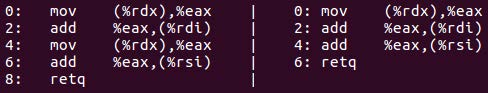
\includegraphics[width=0.9\textwidth]{content/3/chapter12/images/1.jpg}\\
Figure 12.1 – Traversal of std::deque using index versus iterator
\end{center}

It is very important to point out the key difference between designing for performance and optimizing for performance. There is no guarantee that the iterator access to a deque is faster: a particular implementation may, in fact, use the index operator to implement the iterator. Such a guarantee may come only from an optimized implementation. In this chapter, we are interested in the design. The design can't really be "optimized," although, if you talk about an "efficient design," others will likely understand what you mean. The design can allow or prevent certain optimizations, so it is more accurate to talk about "performance-hostile" and "performance-friendly" design (the latter is often called an efficient design). 

In our deque example, the index operator interface is as efficient as it can be for random access, and it treats sequential iteration as a particular case of random access. There is no way for the caller to say, "I will probably ask for the adjacent element next." Conversely, from the existence of the iterator, we can infer that it is likely to be incremented or decremented. The implementation is free to make this increment operation more efficient.

Let us take our container example one step further. This time, we consider a custom container that functions essentially as a tree, but, unlike std::set, we do not store the values in the tree nodes. Instead, we store the values in a sequence container (data store), while the tree nodes contain pointers to elements of this container. The tree is essentially an index into the data store, so it needs a custom comparison function: we want to compare the values, not the pointers.

\hspace*{\fill} \\ %插入空行
\noindent
\textbf{02\_index\_tree.C}
\begin{lstlisting}[style=styleCXX]
template<typename T> struct compare_ptr {
	bool operator()(const T* a, const T* b) const {
		return *a < *b;
	}
};
template <typename T> class index_tree {
	public:
	void insert(const T& t) { 
		data_.push_back(t);
		idx_.insert(&(data_[data_.size() - 1]));
	}
	private:
	std::set<T*, compare_ptr<T>> idx_;
	std::vector<T> data_;
};
\end{lstlisting}

When a new element is inserted, it is added to the end of the data store, while the pointer is added to the appropriate place in the index as determined by the comparison of the elements. Why would we choose such implementation over std::set? In some cases, we may have requirements that force our hand: for example, the data store may be a memory-mapped file on a disk. In other cases, we may choose this implementation for performance benefits, even though at first glance, the extra memory use and the indirect access to elements through the pointer should degrade the performance. 

To see the performance advantage of this indexed tree container, let us examine the operation that does the search for an element that satisfies a given predicate. We can do this search easily, assuming our container provides iterators that simply iterate over the index set; the dereference operator should return the indexed element, not the pointer:

\hspace*{\fill} \\ %插入空行
\noindent
\textbf{02\_index\_tree.C}
\begin{lstlisting}[style=styleCXX]
template <typename T> class index_tree {
	using idx_t = typename std::set<T*, compare_ptr<T>>;
	using idx_iter_t = typename idx_t::const_iterator;
	public:
	class const_iterator {
		idx_iter_t it_;
		public:
		const_iterator(idx_iter_t it) : it_(it) {}
		const_iterator operator++() { ++it_; return *this; }
		const T& operator*() const { return *(*it_); }
		friend bool operator!=(const const_iterator& a,
		const const_iterator& b) {
			return a.it_ != b.it_;
		}
	};
	const_iterator cbegin() const { return idx_.cbegin(); }
	const_iterator cend() const { return idx_.cend(); }
	…
};
\end{lstlisting}

To determine whether a value that meets certain requirements has been stored in the container, we can simply iterate over the entire container and check the predicate for every value:

\begin{lstlisting}[style=styleCXX]
template <typename C, typename F> bool find(const C& c, F f) {
	for (auto it = c.cbegin(), i0 = c.cend(); it != i0; ++it) {
		if (f(*it)) return true;
	}
	return false;
}
\end{lstlisting}

What information do we supply to the container when we access it using the iterators, as we did just now? Just like before, we tell it that we intend to access the next element, every time. We do not tell it anything about the reason we are doing this. Does the intent matter? In this case, very much so. Look carefully at what we really need to do: we need to access every element in the container until we find one that meets the given condition. If this seems like restating the same thing, you are not being pedantic enough. Nowhere in this statement of requirement did we say that we want to access container elements in order, only that we need to iterate over all of them. If we had an API call that tells the container to check all elements but does not require any particular order, the container implementation would be free to optimize the access order. For our indexed container, the optimal access order is to iterate over the data store vector itself: this provides the best memory access pattern (sequential access). The actual order of the elements in the store is, in our case, the order in which they were added, but it does not matter: all we are asking to return is a Boolean value; we do not even ask where the matching element is located. To put it another way, while there may be multiple elements that satisfy the condition, the caller wants to know whether at least one such element exists. We did not ask for the value of the element or for any specific element: this is the request to "find any," not "find first." 

Here is the version of the interface that allows the caller to supply all the relevant information and a possible implementation:

\hspace*{\fill} \\ %插入空行
\noindent
\textbf{02\_index\_tree.C}
\begin{lstlisting}[style=styleCXX]
template <typename T> class index_tree {
	…
	template <typename F> bool find(F f) const {
		for (const T& x : data_) {
			if (f(x)) return true;
		}
		return false;
	}
};
\end{lstlisting}

Is it faster? Again, a benchmark can answer. The difference is more pronounced if the value is not found or found rarely:

\hspace*{\fill} \\ %插入空行
\begin{center}
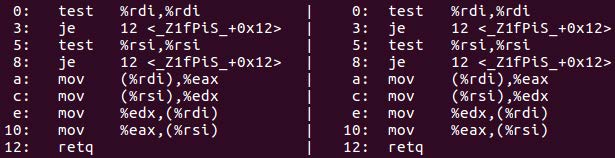
\includegraphics[width=0.9\textwidth]{content/3/chapter12/images/2.jpg}\\
Figure 12.2 – Search in an indexed data store using iterators vs. find() member function
\end{center}

Once again, it is very important to take a step back and reevaluate this example as a lesson for software design instead of a particular optimization technique. In this context, it is not important that our find() member function is so much faster than the iterator-based search. What is important at the design stage is that it might be faster with the appropriate implementation. The reason it might be faster is the knowledge of the caller's intent. 

Compare the information supplied by the caller using non-member vs. member find(). When the non-member find() function calls the container interface, we tell the container, "let me see the values of all container elements, one by one, in order." We don't actually need most of this, but that's the information we give the container because that's the only information we can channel through the iterator interface. On the other hand, the member find() allows us to make the following request: "examine all elements in any order and tell me if there is at least one that matches this condition." This request imposes much fewer restrictions: it is a high-level request that leaves the details to the container itself. In our example, the implementer took advantage of this freedom to provide much better performance.

At the design stage, you will likely not know that such optimized implementation is possible. The very first implementation of the member find() might as well run the iterator loop or call std::find\_if. It is also possible that you will never get to optimizing this function because, in your applications, it is rarely called and is not a performance bottleneck. But software systems tend to live longer than you expect, and fundamental redesign is difficult and time-consuming. A good system architecture should not restrict the evolution of the system for years, sometimes decades, even as new features are added and performance requirements change.

Again, we have seen the difference between a performance-friendly and a performance-hostile design. The same principle applies, of course, to interactions between system components and is not limited to the classes: when designing a component that responds to a request or provides a service, allow the requestor to supply all relevant information, in particular, to express the intent behind the request.

This is a more controversial guideline for several reasons. First of all, it explicitly goes against the popular approach to class design: never implement a (public) member function for a task that does not require privileged access and can be implemented entirely through an existing public API. There are several ways we can reason about this. First of all, one can say that "can be implemented ten times slower" does not really qualify as "can be implemented," so the guideline does not apply. The counterpoint is that at the design stage, you may not even know that you need this performance. The other important rule that we may be violating is "do not optimize prematurely," although this rule should not be taken simplistically: in particular, a reasonable proponent of this rule will often add, "but do not pessimize prematurely either." The latter, in the context of design, means making design decisions that cut off future optimization opportunities. 

The use of the maximum information principle (or information-rich interface) is, thus, a matter of balance and sound judgment. Consider that, in general, violating this guideline is not nearly as maleficent as not following the previous rule: if your interface or contract exposes unnecessary information, it is very hard to take it back from all the clients who came to rely on it. On the other hand, if your interface does not allow the client to supply the relevant intent information, the client may be forced into an inefficient implementation. But nothing will break after you add the more information-rich interface later, and the clients can transition to this interface as needed.

The decision about whether to provide a more information-rich interface upfront, thus, hinges on several factors: 

\begin{itemize}
\item 
How likely is it that this component or this interaction between components is going to be performance-critical? While guessing about the performance of a particular code is to be discouraged, you usually know the general requirements for the components in question: a database that is accessed millions of times per second is likely to be a performance bottleneck somewhere, while the system that serves employee addresses for paychecks twice a month can be designed conservatively and optimized later if needed.

\item 
How broad is the impact of this design decision? In particular, if the inefficient implementation proliferates, how entrenched would it be by the time we add a new, higher-level interface? A class that is used once or twice can be easily updated along with its clients; a communication protocol that will become the standard for the entire system and will be used in a restful API that stores messages on disk for weeks and months should have extensibility built into it from the start, including an option for future information-rich requests.
\end{itemize}

Often, these choices are not clear-cut and rely on the designer's intuition tempered with knowledge and experience. This book can help with the former, and practice takes care of the latter. 

As you have seen throughout this section, we often focus on the interfaces and data organization when considering the performance implications of different design decisions. In the following two sections, we will turn explicitly to these two subjects, starting with the interface design.








